% ==============================================================
%  laporan.tex  –  Root file Laporan Tugas Besar IF3170
%  Compile: pdflatex -> pdflatex  (atau latexmk -pdf laporan)
% ==============================================================

\documentclass[12pt,a4paper]{article}

% ── Encoding & Font ───────────────────────────────────────────
\usepackage[utf8]{inputenc}
\usepackage[T1]{fontenc}

% ── Layout ────────────────────────────────────────────────────
\usepackage[margin=2.5cm,headheight=16pt,headsep=18pt]{geometry}
\usepackage{fancyhdr}
\usepackage[section]{placeins}   % FloatBarrier per section
\usepackage{needspace}
\usepackage{float}
\usepackage{ragged2e}

% ── Grafik & Warna ────────────────────────────────────────────
\usepackage{graphicx}
\graphicspath{{./}{docs/}}
\usepackage{xcolor}

% ── Tabel ─────────────────────────────────────────────────────
\usepackage{booktabs}
\usepackage{tabularx}
\usepackage{multirow}
\usepackage{array}

% ── Matematika ────────────────────────────────────────────────
\usepackage{amsmath}
\usepackage{amssymb}

% ── Source Code ───────────────────────────────────────────────
\usepackage{listings}
\usepackage{inconsolata}
\lstset{
    language=Python,
    basicstyle=\ttfamily\footnotesize,
    keywordstyle=\bfseries\color{blue!70!black},
    stringstyle=\color{orange!80!black},
    commentstyle=\itshape\color{green!50!black},
    emphstyle=\bfseries,
    breaklines=true,
    frame=single,
    showstringspaces=false,
    columns=fullflexible,
    aboveskip=4pt,
    belowskip=4pt,
    floatplacement=htbp,
    captionpos=b,
}
\renewcommand{\lstlistingname}{Cuplikan}

% ── Caption & TikZ ────────────────────────────────────────────
\usepackage{caption}
\usepackage{subcaption}
\usepackage{tikz}
\usetikzlibrary{arrows.meta,positioning}

% ── Strikethrough (surat pernyataan AI) ───────────────────────
\usepackage[normalem]{ulem}

% ── Hyperlink ─────────────────────────────────────────────────
\usepackage[hidelinks]{hyperref}

% ── Lokalisasi (Bahasa Indonesia) ────────────────────────────
\renewcommand{\contentsname}{Daftar Isi}
\renewcommand{\appendixname}{Lampiran}
\renewcommand{\tablename}{Tabel}
\renewcommand{\figurename}{Gambar}
\renewcommand{\lstlistingname}{Cuplikan}

% ── Tipografi ─────────────────────────────────────────────────
\setcounter{tocdepth}{3}
\setlength{\parindent}{1.5em}
\setlength{\parskip}{0pt}
\raggedbottom
\clubpenalty=10000
\widowpenalty=10000
\displaywidowpenalty=10000

% ── Float tuning ─────────────────────────────────────────────
\renewcommand{\topfraction}{0.9}
\renewcommand{\bottomfraction}{0.8}
\renewcommand{\textfraction}{0.08}
\renewcommand{\floatpagefraction}{0.75}
\captionsetup{font=small,labelfont=bf,labelsep=period,skip=6pt}
\setlength{\textfloatsep}{10pt}
\setlength{\intextsep}{10pt}
\makeatletter\setlength{\@fpsep}{10pt}\makeatother

% ── FloatBarrier sebelum setiap subsection/subsubsection ─────
\AddToHook{cmd/subsection/before}{\FloatBarrier\Needspace{7\baselineskip}}
\AddToHook{cmd/subsubsection/before}{\FloatBarrier\Needspace{5\baselineskip}}

% ── Header / Footer ──────────────────────────────────────────
\pagestyle{fancy}
\fancyhf{}
\fancyhead[L]{IF3170 -- Inteligensi Artifisial}
\fancyhead[R]{\thepage}
\renewcommand{\headrulewidth}{0.4pt}
\renewcommand{\footrulewidth}{0pt}

% ==============================================================
\begin{document}
% ==============================================================

% ── Cover / Halaman Judul ────────────────────────────────────
\hypersetup{pageanchor=false}
\begin{titlepage}
    \centering
    {\Huge\bfseries Laporan Tugas Besar 2\par}
    \vspace{0.5cm}
    {\LARGE\scshape IF3170 Inteligensi Artifisial\par}
    \vspace{0.3cm}
    {\Large\scshape Klasifikasi Pembatalan Pemesanan Penginapan\par}
    \vspace{0.2cm}
    {\Large\scshape dengan Algoritma Supervised Learning\par}
    \vspace{0.3cm}
    {\Large\scshape Tahun Akademik 2026--2027\par}
    \vfill
    
\includegraphics[width=7.5cm,keepaspectratio]{logo-itb.png}\par
    \vfill
    {\large\bfseries Disusun oleh:\par}
    \vspace{0.3cm}
    {\large LalapKaoBole\par}
    \vspace{0.3cm}
    {\large Nicholas Wise Saragih Sumbayak -- 13524037\par}
    {\large Nathan E C Marpaung            -- 13524062\par}
    {\large Kurt Mikhael Purba             -- 13524065\par}
    {\large Aurelia Jennifer Gunawan       -- 13524089\par}
    {\large Amanda Aurellia Salsabila      -- 13524131\par}
    \vfill
    {\large\scshape Laboratorium Inteligensi Artifisial\par}
    {\large\scshape Program Studi Teknik Informatika\par}
    {\large\scshape Sekolah Teknik Elektro dan Informatika\par}
    {\large\scshape Institut Teknologi Bandung\par}
\end{titlepage}

% ── Daftar Isi ───────────────────────────────────────────────
\pagenumbering{arabic}
\hypersetup{pageanchor=true}
{\small\linespread{0.92}\selectfont\tableofcontents}
\clearpage

% ── Bab-bab (masing-masing file terpisah) ───────────────────
% ============================================================
%  Bab 1 – Deskripsi Persoalan (Pendahuluan)
% ============================================================

\section{Pendahuluan}

\subsection{Latar Belakang}
% TODO: Jelaskan konteks dan motivasi pemilihan topik.

\subsection{Rumusan Persoalan dan Tujuan}
% TODO: Rumuskan persoalan klasifikasi dan tujuan tugas besar.

\subsection{Deskripsi Dataset}

\subsubsection{Sumber dan Struktur Dataset}
% TODO: Sebutkan sumber dataset (Kaggle, dsb.), jumlah baris/kolom, format file.

\subsubsection{Atribut dan Tipe Data}
% TODO: Tabel atribut — nama kolom, tipe data, deskripsi singkat.

\subsubsection{Variabel Target}
% TODO: Jelaskan kolom target, distribusi kelas (canceled vs.\ not canceled).

\subsection{Batasan Persoalan}
% TODO: Sebutkan asumsi dan batasan yang digunakan dalam pengerjaan.


\clearpage

% ============================================================
%  Bab 2 – Dasar Teori
% ============================================================

\section{Dasar Teori}

\subsection{Supervised Learning}
% TODO: Definisi, paradigma, hubungan dengan klasifikasi.

\subsection{Klasifikasi}
% TODO: Pengertian umum klasifikasi biner vs.\ multiclass.

\subsection{K-Nearest Neighbors}
% TODO: Deskripsi algoritma, perhitungan jarak, pemilihan k.

\subsection{Decision Tree Learning}

\subsubsection{Iterative Dichotomiser 3 (ID3)}
% TODO: Kriteria information gain, entropy.

\subsubsection{C4.5}
% TODO: Gain ratio, penanganan nilai kontinu dan hilang.

\subsubsection{Classification and Regression Tree (CART)}
% TODO: Gini impurity, pruning.

\subsection{Logistic Regression}

\subsubsection{Regularisasi L1}
\subsubsection{Regularisasi L2}
\subsubsection{Elastic Net}

\subsection{Support Vector Machine}

\subsubsection{Kernel Linear}
\subsubsection{Kernel Polinomial}
\subsubsection{Kernel Gaussian (RBF)}

\subsection{Bayesian Network (Naive Bayes)}
% TODO: Teorema Bayes, asumsi conditional independence, Laplace smoothing.

\subsection{Validasi dan Metrik Evaluasi}
% TODO: Train-test split, k-fold CV, accuracy, precision, recall, F1, ROC-AUC.


\clearpage

% ============================================================
%  Bagian 3 – Pembahasan Metodologi
% ============================================================

\section{Pembahasan Metodologi}

\subsection{Eksplorasi Data (EDA)}

Eksplorasi dimulai dengan memeriksa tipe data, kelengkapan nilai, duplikasi, dan nilai yang tidak valid. Data latih dan data uji diperiksa secara terpisah. Keduanya memiliki nilai hilang pada delapan fitur yang sama. Jumlah nilai hilang paling banyak terdapat pada \texttt{num\_children}, yaitu 3.035 pada data latih dan 747 pada data uji. Temuan ini menjadi dasar untuk menentukan penanganan nilai hilang sebelum pelatihan.

Distribusi target hanya dapat diperiksa pada data latih. Dari 27.373 pemesanan, 18.404 tidak dibatalkan (67,23\%) dan 8.969 dibatalkan (32,77\%). Karena jumlah pemesanan di kedua kelas berbeda, skor F1 makro digunakan agar kinerja pada masing-masing kelas mendapat bobot yang sama.

Eksplorasi juga mencakup sebaran fitur numerik, frekuensi kategori, hubungan antarfitur, dan pola berdasarkan waktu kedatangan. Untuk fitur seperti jeda pemesanan, tarif per malam, dan kanal pemesanan, sebaran pada data latih dapat dibandingkan menurut status pembatalan. Perbandingan ini menunjukkan asosiasi, bukan sebab pembatalan.

% ----------------------------------------------------------
\subsection{Data Cleaning}

\subsubsection{Penanganan Nilai Hilang}
% TODO: Strategi imputasi (mean, median, modus, drop) beserta alasan.

\subsubsection{Penanganan Data Duplikat}
% TODO: Metode deteksi dan penghapusan duplikat.

\subsubsection{Penanganan Data Tidak Valid}
% TODO: Outlier, nilai negatif pada kolom non-negatif, dsb.

% ----------------------------------------------------------
\subsection{Data Transformation}

\subsubsection{Encoding Fitur Kategorikal}
% TODO: One-hot encoding, label encoding — alasan pemilihan per fitur.

\subsubsection{Normalisasi dan Standardisasi Fitur Numerik}
% TODO: Min-max scaling vs.\ Z-score — alasan pemilihan per algoritma.

\subsubsection{Penanganan Ketidakseimbangan Kelas}
% TODO: SMOTE, undersampling, class weight — metode yang dipilih dan alasannya.

% ----------------------------------------------------------
\subsection{Feature Selection}
% TODO: Metode (filter/wrapper/embedded), fitur yang dipilih, alasan.

\subsection{Dimensionality Reduction}
% TODO: PCA atau lainnya — apakah diterapkan, mengapa.

% ----------------------------------------------------------
\subsection{Implementasi Model}

\subsubsection{K-Nearest Neighbors}
% TODO: Deskripsi kelas KNN — atribut, metode, kompleksitas.
% Contoh template:
%
% \paragraph{Kelas \texttt{KNNClassifier}}
% Kelas ini mengimplementasikan algoritma \textit{K-Nearest Neighbors} dari awal (\textit{from scratch}).
% Atribut dan metode utama dijelaskan berikut.
%
% \begin{lstlisting}[caption={Implementasi KNNClassifier}, label={lst:knn}]
% # tempel source code di sini
% \end{lstlisting}

\subsubsection{Decision Tree Learning}
% TODO: ID3 / C4.5 / CART — kelas, metode rekursi, kriteria split.

\subsubsection{Logistic Regression}
% TODO: Gradient descent, fungsi sigmoid, regularisasi.

\subsubsection{Support Vector Machine}
% TODO: Optimasi dual, kernel trick, parameter C dan gamma.

\subsubsection{Bayesian Network (Naive Bayes)}
% TODO: Estimasi prior dan likelihood, Laplace smoothing.

\subsection{Implementasi Pembanding dengan scikit-learn}
% TODO: Konfigurasi parameter scikit-learn yang dipakai sebagai baseline.

\subsection{Penyimpanan dan Pemuatan Model}
% TODO: Format simpan model (pickle, joblib, dsb.) dan cara memuatnya.


\clearpage

\section{Eksperimen dan Analisis}

\subsection{Rancangan Eksperimen}

\subsubsection{Data Training dan Data Test}

Berkas \texttt{train.csv} berisi 27.373 pemesanan berlabel dengan 17 fitur (14
numerik dan 3 kategorikal), sedangkan \texttt{test.csv} tidak berlabel dan hanya
dipakai untuk menghasilkan prediksi \textit{submission}. Kedua berkas diproses
terpisah, yaitu seluruh parameter \textit{preprocessing} dipelajari dari data
latih lalu diterapkan pada data uji tanpa digabung.

Sekitar 67\% pemesanan pada data latih tidak dibatalkan sehingga akurasi
\textit{baseline} sudah 0,675 dan evaluasi perlu memakai \textit{Macro F1}.
\texttt{days\_before\_arrival} paling berkorelasi dengan pembatalan ($0{,}44$)
sehingga makin jauh hari pemesanan dibuat, makin besar peluang batal, sedangkan
\texttt{special\_requests} berkorelasi negatif ($-0{,}26$). Dari fitur
kategorikal, \texttt{booking\_channel} paling membedakan, yaitu \textit{Online Travel Agent} paling sering batal (36\%), \textit{Corporate} jarang (12\%), dan
\textit{Complimentary} tidak pernah batal. Pembatalan juga berubah mengikuti
bulan, misalnya sekitar 47\% pada Agustus sampai Oktober 2024 tetapi hanya 3\%
pada Januari 2024.

\subsubsection{Pembagian Data dan Validasi}

Pembagian data memakai \texttt{StratifiedGroupKFold} dengan 5 \textit{fold},
\textit{seed} 42, dan pengacakan. Stratifikasi menjaga proporsi kelas batal
sekitar 33\% pada tiap \textit{fold}, sedangkan pengelompokan menjaga baris yang
identik tetap berada pada satu sisi pembagian. Fold pertama (20\% data) dipakai sebagai
data validasi untuk memilih konfigurasi tiap model, dan seluruh model memakai
fold yang sama agar hasilnya sebanding. Evaluasi akhir memakai \textit{5-fold cross-validation} penuh dengan
seluruh langkah \textit{preprocessing} dan pelatihan diulang pada tiap
\textit{fold}, dan hasilnya dilaporkan sebagai rata-rata dan simpangan baku.
Model akhir untuk \textit{submission} dilatih ulang pada seluruh \texttt{train.csv}.

\subsubsection{Konfigurasi Parameter}

Tabel~\ref{tab:param} merangkum konfigurasi terpilih tiap model. Nilai tersebut
dipilih pada data validasi, kecuali faktor \textit{oversampling} C4.5 yang
dipilih dengan validasi silang di dalam data latih.

\begin{table}[H]
\centering
\small
\caption{Konfigurasi terpilih tiap model}
\label{tab:param}

\begin{tabularx}{\textwidth}{@{}lX@{}}
\toprule
Model & Konfigurasi \\
\midrule
KNN & Standardisasi, $k=31$, bobot \texttt{distance} \\
C4.5 & \textit{Gain ratio}, \textit{Reduced Error Pruning} (80\% data pembentuk pohon dan 20\% data \textit{pruning}), \textit{oversampling} kelas batal 2,0 kali, tanpa imputasi, ditambah fitur turunan \\
\textit{Logistic Regression} & \textit{Gradient ascent}, $\lambda=0{,}001$, laju belajar 0,1 \\
SVM & SMO dengan kernel linear, dilatih pada 1.000 baris karena matriks kernel penuh membutuhkan memori $O(n^2)$ \\
\textit{Naive Bayes} & \textit{Binning} 20 kuantil untuk fitur kontinu, $\alpha=2$ \\
\bottomrule
\end{tabularx}
\end{table}

\subsubsection{Metrik Evaluasi}

Metrik dihitung dengan \texttt{sklearn.metrics} dari \textit{confusion matrix}.

\begin{itemize}
    \item \textit{Macro F1} adalah metrik utama, sama dengan metrik
        \textit{leaderboard} Kaggle. Metrik ini merata-ratakan $F_1$ kelas batal
        dan tidak batal sehingga kedua kelas berbobot sama.
    \item \textit{Accuracy}, \textit{precision}, \textit{recall}, dan $F_1$ kelas
        batal sebagai pelengkap. \textit{Accuracy} dibandingkan dengan
        \textit{baseline} 0,675 yang diperoleh jika semua pemesanan ditebak
        tidak batal.
    \item \textit{ROC-AUC} menilai kualitas urutan probabilitas tanpa bergantung
        pada satu \textit{threshold}. Pada C4.5 probabilitas diambil dari
        proporsi kelas pada daun.
    \item \textit{Log-loss} dipakai untuk membandingkan \textit{Logistic Regression} dengan \texttt{scikit-learn}.
\end{itemize}

Selain metrik prediksi, implementasi sendiri dibandingkan dengan
\texttt{scikit-learn} menggunakan metrik yang sama, selisih probabilitas
prediksi, jumlah node pohon, dan waktu pelatihan. Untuk bonus
\textit{cost-sensitive}, ukuran utamanya adalah total biaya
$2\times FP+1\times FN$ dan biaya per pemesanan, dihitung dari prediksi
\textit{out-of-fold} sehingga tiap pemesanan dievaluasi oleh model yang tidak
melatihnya.

\subsection{Hasil Eksperimen dan Visualisasi}

\subsubsection{K-Nearest Neighbors}

Setiap kombinasi skema \textit{scaling}, nilai $k$, dan bobot dievaluasi pada
data validasi. Bobot \texttt{distance} selalu sama atau lebih baik daripada
\texttt{uniform}. Pada bobot \texttt{uniform}, F1 macro turun menjadi sekitar
0,79 saat $k=51$, sedangkan pada \texttt{distance} tetap sekitar 0,83 sampai
0,84 karena tetangga yang jauh hanya mendapat suara kecil. Standardisasi dengan
$k=31$ memberi F1 macro tertinggi (0,841), sedikit di atas \textit{min-max}
(0,838 pada $k=11$), sedangkan transformasi log paling buruk karena
memperkecil perbedaan lead time dan harga yang justru menjadi sinyal kuat.

\subsubsection{Decision Tree Learning}

Pohon C4.5 tanpa \textit{pruning} tumbuh sangat besar karena fitur turunan
menambah banyak kandidat ambang, dengan F1 macro hanya 0,800. \textit{Reduced Error Pruning} memangkasnya menjadi 9.764 simpul dan menaikkan F1 macro menjadi
0,845. Oversampling dua kali lipat menaikkan \textit{recall} dari 0,759 menjadi
0,780 tetapi menurunkan \textit{precision} dari 0,819 menjadi 0,786, sehingga F1
macro sedikit turun menjadi 0,839. Selisih ini masih dalam rentang variasi
antar-\textit{fold} (sekitar 0,01) sehingga oversampling tidak terbukti membantu
maupun merugikan, tetapi tetap dipakai karena faktornya dipilih lewat validasi
silang.

\begin{table}[H]
\centering
\small
\caption{Pengaruh \textit{pruning} dan \textit{oversampling} pada C4.5 (data validasi)}
\label{tab:dtl}

\begin{tabular}{@{}lcc@{}}
\toprule
Konfigurasi C4.5 & Jumlah simpul & F1 macro \\
\midrule
Tanpa \textit{pruning} & 57.264 & 0,800 \\
Dengan \textit{Reduced Error Pruning} & 9.764 & 0,845 \\
Dengan \textit{pruning} dan oversampling & - & 0,839 \\
\bottomrule
\end{tabular}
\end{table}

Pada visualisasi pohon (Gambar~\ref{fig:pohon}), atribut pertama adalah
\texttt{days\_before\_arrival} dengan ambang 148,5 hari, sesuai temuan bahwa
\textit{lead time} paling berhubungan dengan pembatalan. Fitur turunan
\texttt{special\_requests\_missing} juga muncul di level atas.

\begin{figure}[H]
\centering
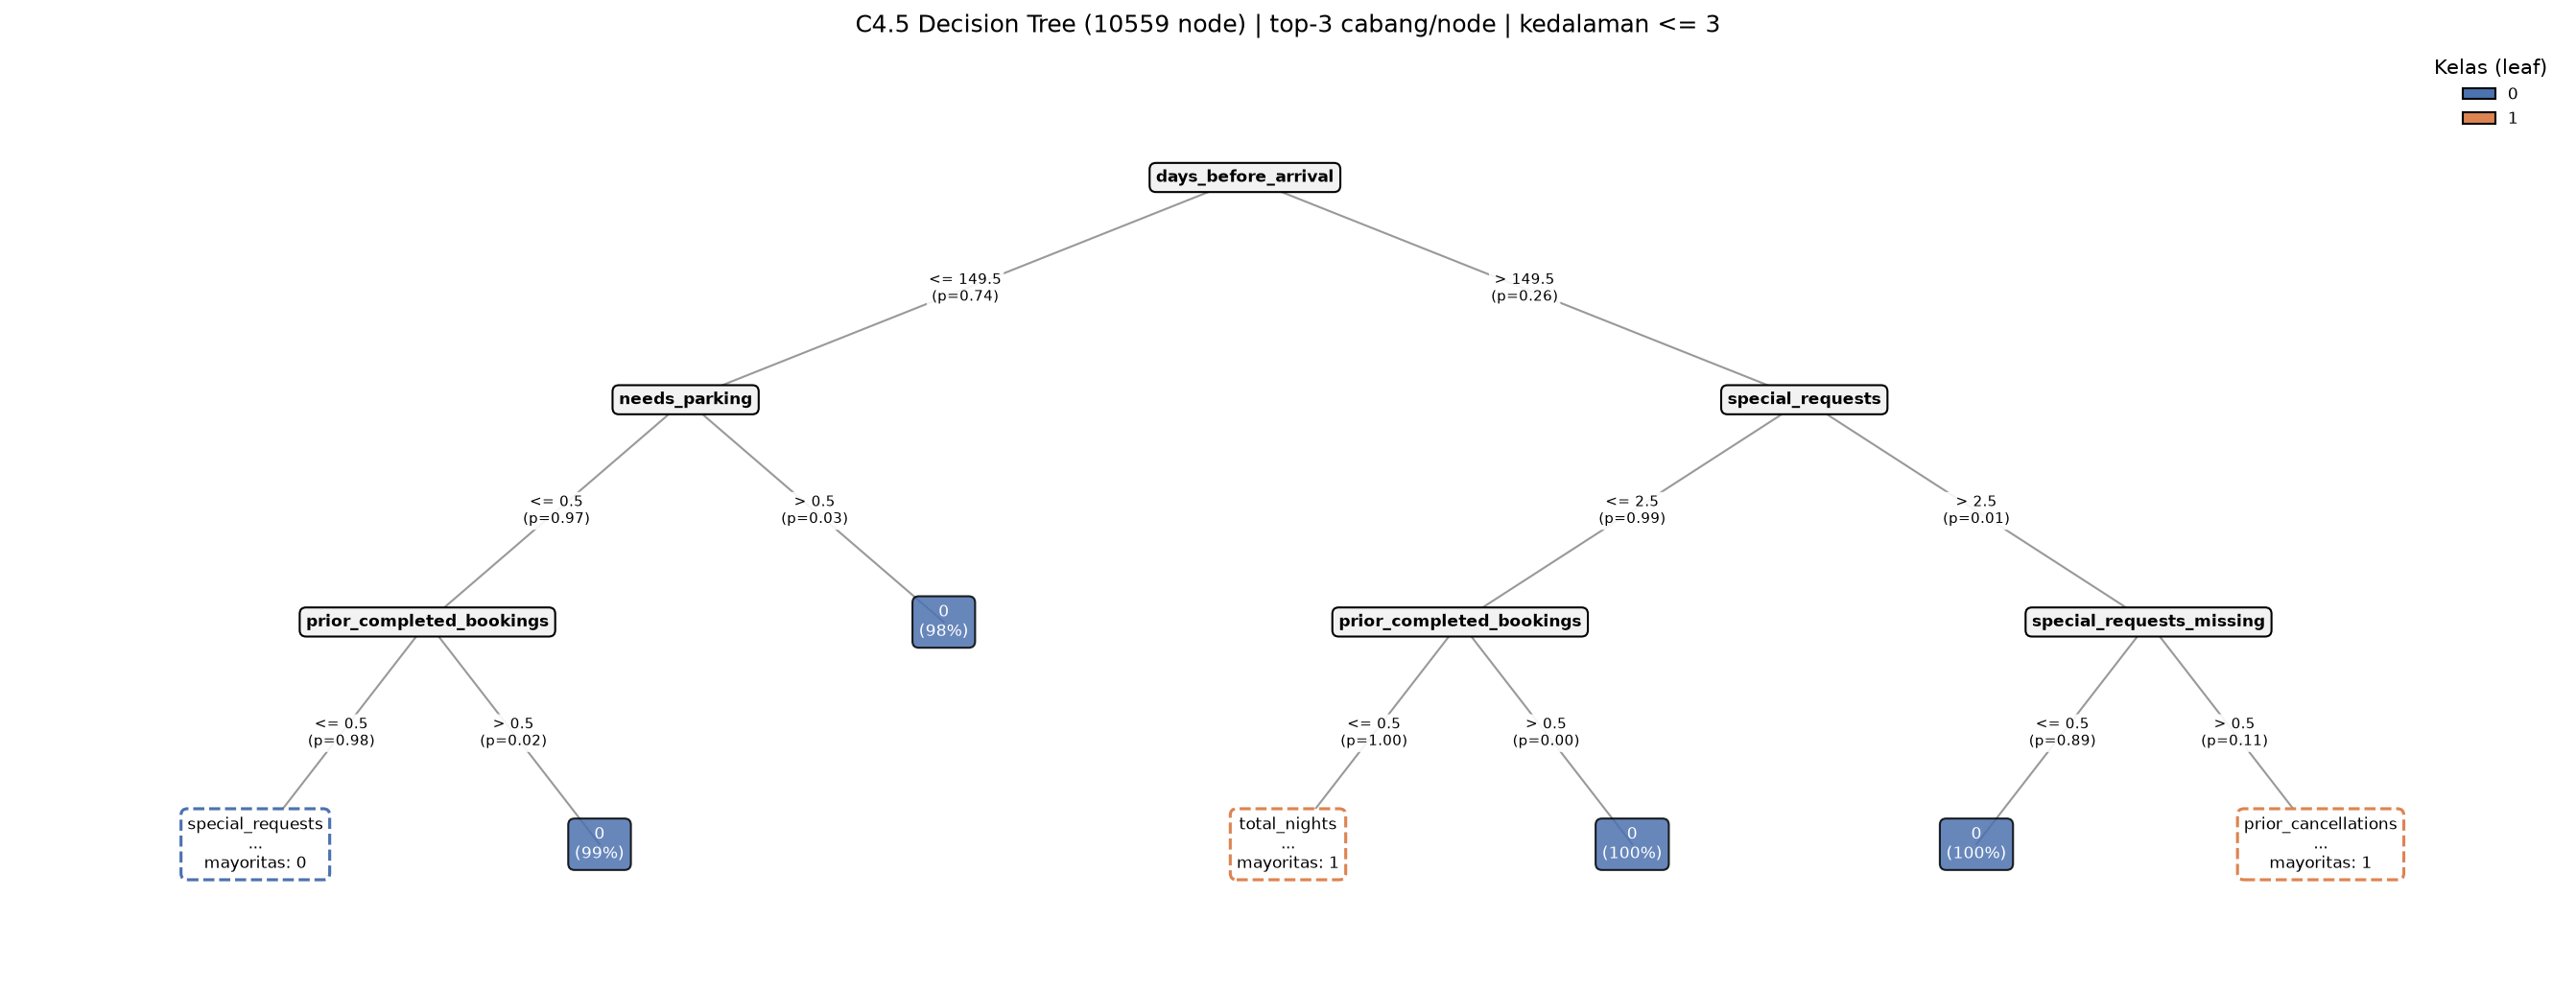
\includegraphics[width=\textwidth]{../output/c45_tree.png}
\caption{Visualisasi tiga level teratas pohon C4.5 (\texttt{top\_n}=3)}
\label{fig:pohon}
\end{figure}

\subsubsection{Logistic Regression}

Empat varian (tanpa penalti, L1, L2, dan \textit{Elastic Net}) dilatih pada
konfigurasi yang setara ($\lambda=0{,}001$). Pengaruh regularisasi sangat kecil
karena $\lambda$ kecil dan data cukup banyak, sehingga keempat varian hampir
tidak berbeda, dengan \textit{accuracy} 0,806 sampai 0,808 dan ROC-AUC 0,865
pada data validasi. Kurva \textit{loss} pelatihan tiap varian ditunjukkan pada
Gambar~\ref{fig:logreg}.

\begin{figure}[H]
\centering
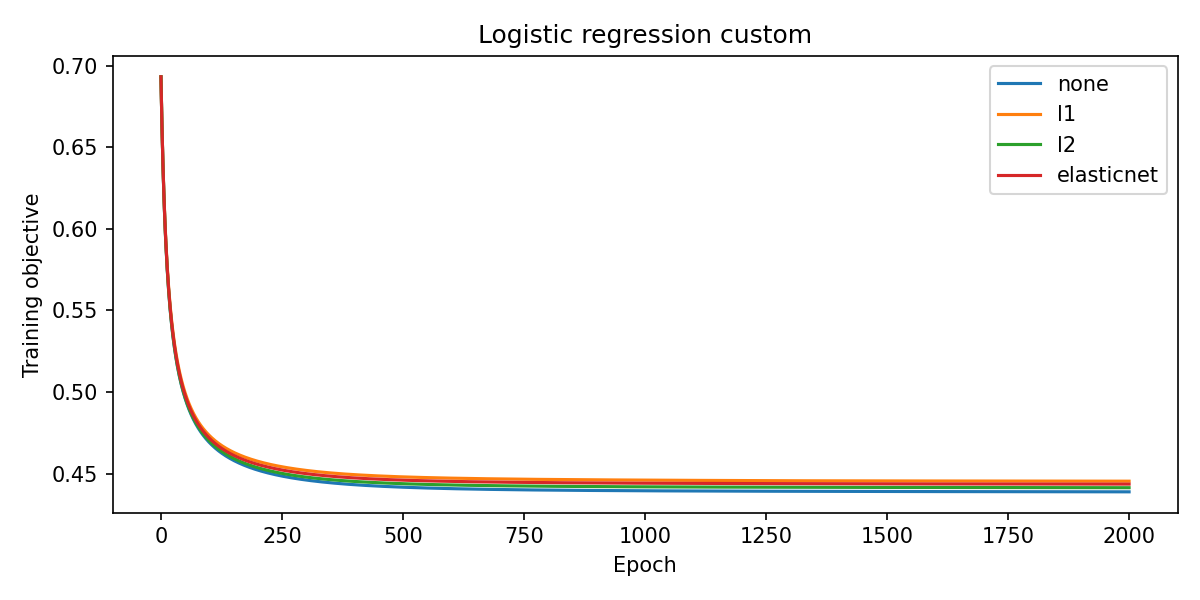
\includegraphics[width=0.8\textwidth]{../output/logreg_loss.png}
\caption{Kurva \textit{loss} pelatihan \textit{Logistic Regression} buatan sendiri}
\label{fig:logreg}
\end{figure}

\subsubsection{Support Vector Machine}
% TODO: Tabel metrik, pengaruh kernel dan C.

\subsubsection{Bayesian Network (Naive Bayes)}
% TODO: Tabel metrik, distribusi probabilitas kelas.

\subsubsection{Perbandingan Antarmodel}

Tabel~\ref{tab:cv} memuat hasil \textit{5-fold cross-validation} dengan
konfigurasi terbaik tiap model.

\begin{table}[H]
\centering
\small
\caption{Hasil \textit{5-fold cross-validation} (rata-rata)}
\label{tab:cv}

\begin{tabular}{@{}lccccc@{}}
\toprule
Model & \textit{Accuracy} & \textit{Precision} & \textit{Recall} & F1 macro & ROC-AUC \\
\midrule
KNN & 0,855 & 0,805 & 0,737 & 0,832 $\pm$ 0,008 & 0,914 \\
C4.5 & 0,853 & 0,795 & 0,744 & 0,830 $\pm$ 0,006 & 0,865 \\
\textit{Logistic Regression} & 0,797 & 0,731 & 0,605 & 0,759 $\pm$ 0,009 & 0,854 \\
SVM & 0,794 & 0,726 & 0,597 & 0,754 $\pm$ 0,010 & 0,843 \\
\textit{Naive Bayes} & 0,781 & 0,687 & 0,610 & 0,744 $\pm$ 0,006 & 0,836 \\
\bottomrule
\end{tabular}
\end{table}

\begin{figure}[H]
\centering
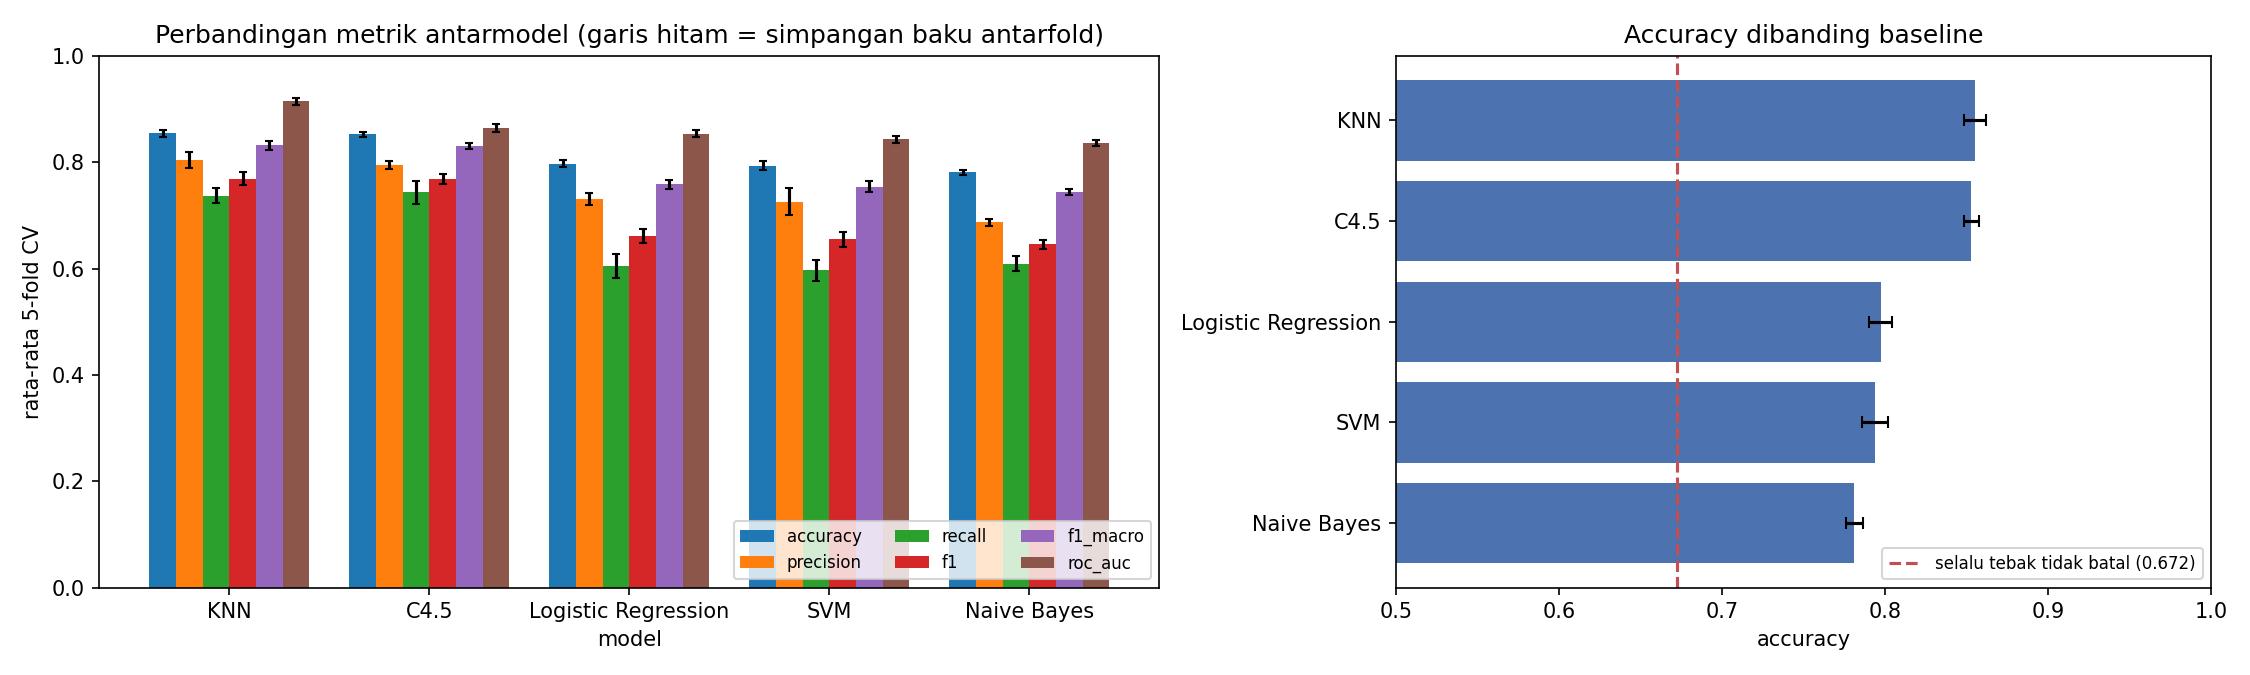
\includegraphics[width=\textwidth]{../output/model_comparison.png}
\caption{Perbandingan metrik antarmodel}
\label{fig:model}
\end{figure}

KNN dan C4.5 memperoleh hasil tertinggi dengan selisih yang jauh lebih kecil dibandingkan
variasi antar-\textit{fold}, sehingga keduanya dapat dianggap setara. Perbedaan
terbesar ada pada ROC-AUC (0,914 untuk KNN dan 0,865 untuk C4.5) karena
probabilitas KNN berasal dari 31 tetangga berbobot jarak sehingga lebih halus,
sedangkan probabilitas C4.5 hanya proporsi kelas pada daun. \textit{Logistic Regression} dan SVM hampir sama karena SVM terbaik memakai kernel linear
sehingga keduanya sama-sama membentuk batas lurus. KNN dan C4.5 unggul karena
dapat menangkap pola nonlinear dan interaksi antarfitur, sedangkan model linear
hanya memberi satu bobot pada tiap fitur. Semua model jauh di atas
\textit{baseline} 0,675, tetapi \textit{recall} hanya 0,60 sampai 0,74
sehingga 26 sampai 40\% pemesanan yang batal belum terdeteksi. Fold pertama
memberi skor tertinggi untuk semua model, kemungkinan karena konfigurasi
dipilih dengan \textit{fold} tersebut, sehingga rata-rata 5 \textit{fold} lebih
dapat dipercaya untuk membandingkan model.

\subsubsection{Cost-Sensitive Classification}

Tabel~\ref{tab:cost} membandingkan prediksi \textit{out-of-fold} pada
\textit{threshold} 0,5 dan 0,667 dengan $C_{FP}=2$ dan $C_{FN}=1$. SVM tidak
disertakan karena skornya bukan probabilitas.

\begin{table}[H]
\centering
\small
\caption{Pengaruh \textit{threshold} \textit{cost-sensitive} terhadap total biaya}
\label{tab:cost}

\begin{tabular}{@{}lcrrr@{}}
\toprule
Model & \textit{Threshold} & $FP$ & $FN$ & Total biaya \\
\midrule
KNN & 0,5 & 1.607 & 2.359 & 5.573 \\
 & 0,667 & 614 & 3.865 & 5.093 \\
C4.5 & 0,5 & 1.722 & 2.299 & 5.743 \\
 & 0,667 & 1.474 & 2.492 & 5.440 \\
\textit{Logistic Regression} & 0,5 & 1.997 & 3.549 & 7.543 \\
 & 0,667 & 839 & 5.311 & 6.989 \\
\textit{Naive Bayes} & 0,5 & 2.488 & 3.503 & 8.479 \\
 & 0,667 & 1.027 & 4.948 & 7.002 \\
\bottomrule
\end{tabular}
\end{table}

Pada semua model, \textit{threshold} 0,667 menurunkan jumlah $FP$ dan menaikkan
jumlah $FN$, dan total biaya ikut turun karena $FP$ berbobot dua kali lipat.
Penurunan terbesar terjadi pada \textit{Naive Bayes} (sekitar 17\%), yang
memiliki $FP$ terbanyak pada \textit{threshold} 0,5, dan terkecil pada C4.5
(sekitar 5\%). KNN memiliki total biaya terendah (5.093), dengan $FP$ turun
dari 1.607 menjadi 614. Perubahan ini memberi pertukaran yang harus
dipertimbangkan, yaitu lebih banyak pemesanan batal yang tidak terdeteksi sebagai
imbalan lebih sedikit risiko \textit{overbooked}.

\begin{figure}[H]
\centering
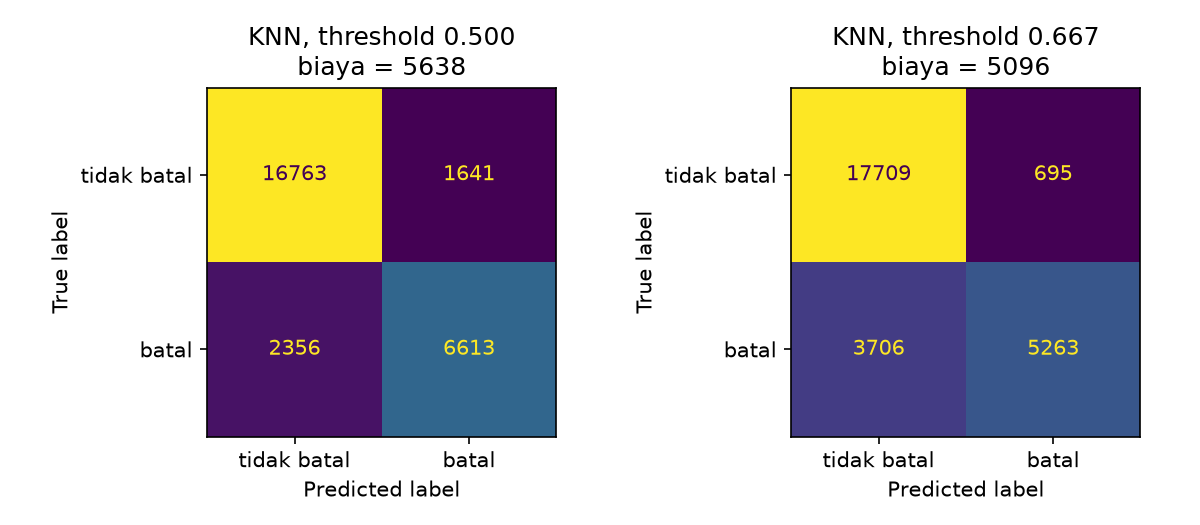
\includegraphics[width=0.8\textwidth]{../output/cost_sensitive_confusion_matrix.png}
\caption{\textit{Confusion matrix} model dengan biaya terendah pada kedua \textit{threshold}}
\label{fig:cost}
\end{figure}

\subsection{Perbandingan Implementasi dengan Pustaka}

\subsubsection{Perbandingan Metrik}

Tiap algoritma dibandingkan dengan padanannya pada \texttt{scikit-learn} pada
data validasi yang sama.

\paragraph{KNN.} Hasil kedua implementasi identik (Tabel~\ref{tab:knn}). Hanya
satu dari 5.474 baris validasi yang probabilitasnya berbeda, dan itu terjadi
karena beberapa tetangga berjarak sama persis di batas tetangga ke-$k$ sehingga
urutan pemilihannya berbeda.

\begin{table}[H]
\centering
\small
\caption{KNN buatan sendiri dan \texttt{scikit-learn} pada data validasi}
\label{tab:knn}

\begin{tabular}{@{}lccc@{}}
\toprule
Model & \textit{Accuracy} & F1 macro & ROC-AUC \\
\midrule
\texttt{KNNClassifier} & 0,863 & 0,841 & 0,923 \\
\texttt{KNeighborsClassifier} & 0,863 & 0,841 & 0,923 \\
\bottomrule
\end{tabular}
\end{table}

\paragraph{Decision Tree.} C4.5 unggul pada F1 macro (Tabel~\ref{tab:dtlsk}),
sedangkan \texttt{scikit-learn} dengan \textit{pruning} memiliki
\textit{recall} (0,846) dan ROC-AUC (0,917) lebih tinggi dengan pohon yang jauh
lebih kecil, tetapi \textit{precision}-nya lebih rendah. Perbedaan ini berasal
dari algoritma yang berbeda, yaitu \textit{gain ratio} dengan cabang per
kategori pada C4.5 dan pemecahan biner dengan \textit{cost-complexity pruning}
pada CART. ROC-AUC C4.5 yang lebih rendah kemungkinan karena banyaknya daun
murni sehingga skor probabilitasnya kurang halus.

\begin{table}[H]
\centering
\small
\caption{C4.5 dan \texttt{scikit-learn} pada data validasi}
\label{tab:dtlsk}

\begin{tabular}{@{}lcc@{}}
\toprule
Model & Jumlah simpul & F1 macro \\
\midrule
C4.5 dengan \textit{Reduced Error Pruning} & 9.764 & 0,845 \\
C4.5 dengan \textit{pruning} dan oversampling & - & 0,839 \\
\texttt{scikit-learn} tanpa \textit{pruning} & - & 0,807 \\
\texttt{scikit-learn}, \texttt{ccp\_alpha}=0,0005 & 389 & 0,825 \\
\bottomrule
\end{tabular}
\end{table}

\paragraph{Logistic Regression.} Selisih metrik antara implementasi sendiri dan
\texttt{scikit-learn} kurang dari 0,002 (Tabel~\ref{tab:logreg}), sehingga
implementasi sendiri dinilai benar.

\begin{table}[H]
\centering
\small
\caption{\textit{Logistic Regression} buatan sendiri dan \texttt{scikit-learn} pada data validasi}
\label{tab:logreg}

\begin{tabular}{@{}llccc@{}}
\toprule
Varian & Implementasi & \textit{Accuracy} & $F_1$ batal & ROC-AUC \\
\midrule
Tanpa penalti & Sendiri & 0,808 & 0,681 & 0,865 \\
 & \texttt{scikit-learn} & 0,806 & 0,680 & 0,865 \\
L1 & Sendiri & 0,806 & 0,678 & 0,865 \\
 & \texttt{scikit-learn} & 0,807 & 0,679 & 0,865 \\
L2 & Sendiri & 0,807 & 0,680 & 0,865 \\
 & \texttt{scikit-learn} & 0,806 & 0,678 & 0,865 \\
\textit{Elastic Net} & Sendiri & 0,807 & 0,680 & 0,865 \\
 & \texttt{scikit-learn} & 0,807 & 0,680 & 0,865 \\
\bottomrule
\end{tabular}
\end{table}

\subsubsection{Analisis Waktu Eksekusi}

Tabel~\ref{tab:waktu} membandingkan waktu pelatihan KNN dan \textit{Logistic
Regression}. Implementasi KNN sendiri sedikit lebih lambat karena belum
memanfaatkan optimasi \textit{library}. Implementasi \textit{Logistic
Regression} sendiri lebih lambat pada L1 dan terutama pada \textit{Elastic Net}
karena memakai \textit{gradient ascent} penuh sampai \textit{loss} stabil,
sedangkan SAGA lebih efisien. Pada varian tanpa penalti, implementasi sendiri
justru lebih cepat.

\begin{table}[H]
\centering
\small
\caption{Waktu pelatihan pada data validasi (detik)}
\label{tab:waktu}

\begin{tabular}{@{}lcc@{}}
\toprule
Model & Sendiri & \texttt{scikit-learn} \\
\midrule
KNN & 3,6 & 2,8 \\
\textit{Logistic Regression}, tanpa penalti & 9,9 & 28,4 \\
\textit{Logistic Regression}, L1 & 9,7 & 4,5 \\
\textit{Logistic Regression}, L2 & 9,6 & 10,2 \\
\textit{Logistic Regression}, \textit{Elastic Net} & 129,4 & 12,0 \\
\bottomrule
\end{tabular}
\end{table}

\subsubsection{Analisis Visualisasi}
% TODO: Plot perbandingan kurva ROC atau confusion matrix berdampingan.

\subsection{Kaggle Submission}
% TODO: Skor leaderboard Kaggle dan konfigurasi model yang dikirim.

\clearpage

\clearpage
\section{Kesimpulan dan Saran}

\subsection{Kesimpulan}

Pada Tugas Besar 2 IF3170 Inteligensi Artifisial, tim berhasil membangun \textit{pipeline} lengkap untuk
memprediksi pembatalan pemesanan penginapan, mulai dari analisis data,
\textit{preprocessing}, pelatihan, hingga evaluasi. Lima algoritma, yaitu KNN,
\textit{Decision Tree Learning} (C4.5), \textit{Logistic Regression}, SVM, dan
\textit{Naive Bayes}, diimplementasikan dari awal menggunakan NumPy dan
dibandingkan dengan scikit-learn. Analisis data menunjukkan bahwa sekitar 33\% pemesanan
dibatalkan dan sekitar 39\% baris memiliki nilai kosong. Oleh karena itu
\textit{preprocessing} disesuaikan dengan kebutuhan tiap algoritma, dan
pembagian data memakai StratifiedGroupKFold agar baris yang identik
tidak berada pada data latih dan validasi sekaligus. Hasil implementasi sendiri
sesuai dengan scikit-learn. KNN dan \textit{Naive Bayes} menghasilkan
probabilitas yang hampir identik, dan selisih metrik \textit{Logistic Regression}
kurang dari 0,002. C4.5 berbeda karena algoritma pembandingnya adalah CART,
tetapi hasilnya tetap sebanding.

Berdasarkan \textit{5-fold cross-validation}, KNN (F1 macro 0,832) dan C4.5
(0,830) memberikan performa terbaik dengan selisih yang lebih kecil daripada
variasi antar-\textit{fold}, sehingga keduanya dapat dianggap setara.
Keduanya unggul karena mampu menangkap pola nonlinear dan interaksi antarfitur,
sedangkan \textit{Logistic Regression} (0,759), SVM berkernel linear (0,754),
dan \textit{Naive Bayes} (0,748) hanya membentuk batas yang lebih sederhana atau
mengasumsikan fitur saling bebas. Menambahkan pohon ketergantungan antarfitur
lewat \textit{Tree Augmented Naive Bayes} (bonus) menaikkan F1 macro
\textit{Naive Bayes} menjadi 0,775, sehingga asumsi independensi memang ikut
menurunkan skornya, tetapi belum cukup untuk menyamai KNN dan C4.5. Seluruh model berada jauh di atas
\textit{baseline} 0,675, tetapi \textit{recall} kelas batal baru mencapai 0,60
sampai 0,74. Pada bonus, penggeseran \textit{threshold} menjadi 0,667 untuk
\textit{cost-sensitive classification} menurunkan total biaya pada semua model,
dengan biaya terendah dicapai KNN (5.093). Visualisasi pohon, video lintasan
parameter \textit{Logistic Regression}, dan graf \textit{Naive Bayes} juga
berhasil dibuat untuk membantu menjelaskan perilaku model.

\subsection{Saran}

Untuk pengembangan lebih lanjut, disarankan mencoba model \textit{ensemble}
seperti \textit{Random Forest} atau \textit{gradient boosting} yang menggabungkan
kelebihan pohon keputusan, serta melakukan \textit{hyperparameter tuning} yang
lebih ekstensif. Rekayasa fitur tambahan, misalnya fitur interaksi untuk model
linear, juga berpotensi meningkatkan \textit{Logistic Regression} dan SVM.
Karena \textit{recall} kelas batal masih rendah, pemilihan \textit{threshold}
yang dioptimalkan langsung terhadap \textit{Macro F1} atau terhadap biaya
dapat dicoba. Pada \textit{Naive Bayes}, TAN menaikkan skor dengan memodelkan
ketergantungan antarfitur, sehingga model yang memodelkan interaksi lebih dari
dua fitur dapat dicoba untuk menyempitkan selisih dengan KNN dan C4.5.

Dari sisi implementasi, SVM masih dilatih pada 1.000 baris karena matriks
kernel penuh membutuhkan memori $O(n^2)$ sehingga perlu teknik seperti
\textit{kernel cache} dan \textit{shrinking} agar dapat memakai seluruh data.
Implementasi \textit{Logistic Regression} dengan \textit{Elastic Net} juga jauh
lebih lambat daripada scikit-learn sehingga dapat dipercepat dengan
laju belajar adaptif atau \textit{solver} yang lebih efisien. Terakhir, laporan
ini belum memuat skor \textit{leaderboard} Kaggle untuk seluruh model, sehingga
pengujian pada data uji perlu dilengkapi untuk memastikan hasil validasi dapat
digeneralisasi.

\clearpage

% ============================================================
%  Bagian 6 – Pembagian Tugas Tiap Anggota Kelompok
% ============================================================

\pagebreak
\section{Pembagian Tugas Tiap Anggota Kelompok}

\begin{table}[ht]
    \centering
    \renewcommand{\arraystretch}{1.5}
    \begin{tabularx}{\textwidth}{@{}p{6.1cm}lX@{}}
        \toprule
        \textbf{Nama Lengkap} & \textbf{NIM} & \textbf{Tugas/Kontribusi} \\
        \midrule
        Nicholas Wise Saragih Sumbayak & 13524037 & Implementasi SVM dan
        Algoritma Bonus,\\
        Nathan E C Marpaung            & 13524062 & Implementasi Logistic
        Regression dan Algoritma Bonus \\
        Kurt Mikhael Purba             & 13524065 & Implementasi Decision Tree
        Learning dan Algoritma Bonus \\
        Aurelia Jennifer Gunawan       & 13524089 & Implementasi KNN \\
        Amanda Aurellia Salsabila      & 13524131 & Implementasi Bayesian
        Network dan Algoritma Bonus\\
        \bottomrule
    \end{tabularx}
    \caption{Pembagian tugas anggota kelompok}
\end{table}


\clearpage

% ============================================================
%  Bagian 7 – Referensi
% ============================================================

\clearpage
\section{Referensi}

% Gunakan format referensi manual atau ganti dengan \bibliography{refs} jika pakai BibTeX.
% Contoh format manual (IEEE style):
%
% \begin{enumerate}
%     \item T. Cover and P. Hart, ``Nearest neighbor pattern classification,''
%           \textit{IEEE Trans.\ Inf.\ Theory}, vol.\ 13, no.\ 1, pp.\ 21--27, Jan.\ 1967.
%     \item C. M. Bishop, \textit{Pattern Recognition and Machine Learning}.
%           New York, NY, USA: Springer, 2006.
% \end{enumerate}

\begin{enumerate}
    % TODO: Tambahkan referensi di sini.
\end{enumerate}


\clearpage

% ============================================================
%  Bagian 8 – Lampiran (Form Penggunaan Generative AI)
% ============================================================

\clearpage
\section{Lampiran}
\subsection{Form Penggunaan \textit{Generative} AI}

\begin{center}
    {\large\bfseries SURAT PERNYATAAN PENGGUNAAN AI\par}
\end{center}
\vspace{-0.3em}
\noindent Dengan ini, \sout{saya}/kami*:

\begin{tabular}{@{}l@{\hspace{1.2em}}l@{\hspace{0.8em}}p{0.62\textwidth}@{}}
    Nama/NIM           & : & Nicholas Wise Saragih Sumbayak/13524037, Nathan E C Marpaung/13524062,
                             Kurt Mikhael Purba/13524065, Aurelia Jennifer Gunawan/13524089,
                             Amanda Aurellia Salsabila/13524131 \\
    Fakultas/Sekolah   & : & STEI-K \\
    Kode Mata Kuliah   & : & IF3170 \\
    Nama Mata Kuliah   & : & Inteligensi Artifisial \\
    Judul Tugas/Proposal & : & Tugas Besar 2 \\
\end{tabular}

\vspace{0.6em}
\noindent Menyatakan bahwa \sout{saya}/kami* \underline{menggunakan/tidak menggunakan}* AI dalam pengerjaan
maupun penyusunan luaran tugas pada mata kuliah yang tertulis di atas.

\vspace{0.4em}
\noindent Jika Ya, maka alat AI/kecerdasan buatan yang digunakan adalah:

\vspace{0.4em}
\begin{table}[H]
    \centering
    \small
    \renewcommand{\arraystretch}{1.15}
    \begin{tabularx}{\textwidth}{|>{\raggedright\arraybackslash}X|c|>{\centering\arraybackslash}p{2.6cm}|}
        \hline
        \multicolumn{1}{|c|}{\textbf{Lingkup Pekerjaan}} & \textbf{Digunakan?} & \textbf{Tingkat Penggunaan} \\
        \hline
        \textbf{Pemeriksaan Ejaan:} menggunakan tools seperti Grammarly, Paperpal, DeepL,
        Quillbot, Grammarbot, LanguageTool, ProWritingAid, ChatGPT, Google Gemini,
        atau sejenisnya. & & \\
        \hline
        \textbf{Pembuatan Teks:} menggunakan tools seperti ChatGPT, Gemini, Paperpal,
        Copilot, GrammarlyGO, WordAI, WriteSonic, Jasper, Jenni AI, atau sejenisnya. & & \\
        \hline
        \textbf{Bantuan Diskusi dalam Penyusunan Konten:} menggunakan tools seperti
        ChatGPT, Gemini, Copilot, Perplexity, Jenni AI, Zoom-Companion, atau sejenisnya. & & \\
        \hline
        \textbf{Pembuatan Gambar, Video, dan/atau Grafik:} menggunakan tools seperti
        Craiyon, DALL-E, Midjourney, Stable Diffusion, Microsoft Designer, Gemini, Canva AI,
        atau sejenisnya. & & \\
        \hline
        \textbf{Lainnya, Jelaskan:}\vspace{1.6em} & & \\
        \hline
    \end{tabularx}
\end{table}

\noindent \sout{Saya}/Kami* juga menyatakan bahwa setiap penggunaan AI/kecerdasan buatan yang
dilakukan pada mata kuliah tersebut telah dinyatakan di dalam surat ini.

\vspace{0.5em}
\hfill\begin{minipage}{6.5cm}
    \raggedleft
    Bandung, \rule{3cm}{0.4pt}\par
    \vspace{1.8cm}
    \rule{5cm}{0.4pt}\par
    Nama dan NIM
\end{minipage}



% ==============================================================
\end{document}
